%!TEX program = xelatex
%!TEX spellcheck = en_GB
\documentclass[final]{report}
% Include all project wide packages here.
%\usepackage{fullpage}
\usepackage[a4paper,margin=2.5cm,top=2cm]{geometry}
\usepackage{polyglossia}
\setmainlanguage{english}
\usepackage{csquotes}
\usepackage{graphicx}
\usepackage{pdfpages}
\usepackage{caption}
\usepackage[list=true]{subcaption}
\usepackage{float}
\usepackage{standalone}
\usepackage{import}
\usepackage{tocloft}
\usepackage{wrapfig}
\usepackage{authblk}
\usepackage{array}
\usepackage{booktabs}
\usepackage[title,titletoc]{appendix}
\usepackage{fontspec}
\usepackage{pgfplots}
\usepackage{tikz}
\usepackage[binary-units=true]{siunitx}
\usepackage{units}
\usepackage{amsmath}
\usepackage{mathtools}
\usepackage{unicode-math}
\usepackage{rotating}
\usepackage{titlesec}
\usepackage{titletoc}
\usepackage{blindtext}
\usepackage{color}
\usepackage{enumitem}
\usepackage{tabularx}
\usepackage{titling}
\usepackage[%
siunitx,
fulldiodes,
europeanvoltages,
europeancurrents,
europeanresistors,
americaninductors,
smartlabels]{circuitikz}

\newcommand{\matlab}{{\textsc{matlab }}}

\usetikzlibrary{calc}
\usetikzlibrary{positioning}
\usetikzlibrary{automata}
\usetikzlibrary{arrows.meta}

\tikzstyle{every state}=[fill=tu-cyan,align=center,draw=black,line width=1pt,node distance=3cm,minimum width = 1.8cm]%for FSMs casper
\tikzstyle{every initial by arrow}=[initial text={Reset}]
\newcommand{\setpathasarrows}{\tikzstyle{every path}=[auto,line width=1.5pt,line cap=round,line join=round]}

\pgfplotsset{compat=newest}
\pgfplotsset{plot coordinates/math parser=false}
\usetikzlibrary{plotmarks}
\usepgfplotslibrary{patchplots}
\newlength\figureheight
\newlength\figurewidth

\tikzset{every axis/.style={xticklabel style={align=right}}}

\usepackage[
%backend=bibtex,
backend=biber,
	texencoding=utf8,
bibencoding=utf8,
style=numeric,
citestyle=numeric,
    sortlocale=en_US,
    language=auto,
    backref=true,
    abbreviate=false,
    date=edtf,
    seconds=true
]{biblatex}


\usepackage{listings}
\newcommand{\includecode}[4][c]{\lstinputlisting[caption=#2, escapechar=, style=#1,label=#4]{#3}}
\newcommand{\superscript}[1]{\ensuremath{^{\textrm{#1}}}}
\newcommand{\subscript}[1]{\ensuremath{_{\textrm{#1}}}}


\newcommand{\chapternumber}{\thechapter}
\renewcommand{\appendixname}{Appendix}
\renewcommand{\appendixtocname}{Appendices}
\renewcommand{\appendixpagename}{Appendices}


\setlist[enumerate]{labelsep=*, leftmargin=1.5pc}
\setlist[enumerate,1]{label=\arabic*., ref=\arabic*}
\setlist[enumerate,2]{label=\arabic*.,ref=\theenumi.\arabic*}
\setlist[enumerate,3]{label=\arabic*., ref=\theenumii.\arabic*}

%\setcounter{chapter}{-1} %start chapter numbers with 0

\usepackage{xr-hyper}
\usepackage[hidelinks]{hyperref} %<--------ALTIJD ALS LAATSTE
\usepackage[nameinlink,noabbrev,capitalise]{cleveref} %<------- Clever Ref moet na hyperref
\crefname{app}{Appendix}{Appendices}
%\renewcommand{\familydefault}{\sfdefault}


\setmainfont{Myriad Pro}[Ligatures={Common,TeX}]
\setmathfont{Asana Math}
\setmonofont[Scale=0.9]{Lucida Console}
\newfontfamily\headingfont{Minion Pro}[Ligatures={Common,TeX}]


%Design colors
\definecolor{accent1}{RGB}{0,100,200}
\definecolor{accent2}{RGB}{0,50,100}
\definecolor{tu-cyan}{RGB}{0,166,214}

\newcommand{\hsp}{\hspace{20pt}}
\titleformat{\chapter}[hang]{\Huge\headingfont}{\chapternumber\hsp\textcolor{accent2}{|}\hsp}{0pt}{\Huge\headingfont}

\titleformat{name=\chapter,numberless}[hang]{\Huge\headingfont}{\hsp\textcolor{accent2}{|}\hsp}{0pt}{\Huge\headingfont}

\titleformat{\section}[block]{\LARGE\headingfont}{\arabic{chapter}.\arabic{section}}{0.4em}{}
\titleformat{\subsection}[block]{\Large\headingfont}{\arabic{chapter}.\arabic{section}.\arabic{subsection}}{0.4em}{}
\titleformat{\subsubsection}[block]{\large\headingfont}{\arabic{chapter}.\arabic{section}.\arabic{subsection}.\arabic{subsubsection}}{0.4em}{}
\renewcommand{\arraystretch}{1.2}
\renewcommand{\baselinestretch}{1.25} 

\renewcommand\cfttoctitlefont{\headingfont\Huge}
\renewcommand\cftloftitlefont{\headingfont\Huge}
\renewcommand\cftlottitlefont{\headingfont\Huge}
\setcounter{lofdepth}{2}
\setcounter{lotdepth}{2}


\setlength{\parindent}{0pt}
\setlength{\parskip}{1em}


%SIuntix settings:
%default: 0V to 10V
%custom: 0 - 10V
\sisetup{range-phrase=--}
\sisetup{range-units=single}
\DeclareSIUnit\years{years}

%For code listings
\definecolor{black}{rgb}{0,0,0}
\definecolor{browntags}{rgb}{0.65,0.1,0.1}
\definecolor{bluestrings}{rgb}{0,0,1}
\definecolor{graycomments}{rgb}{0.4,0.4,0.4}
\definecolor{redkeywords}{rgb}{1,0,0}
\definecolor{bluekeywords}{rgb}{0.13,0.13,0.8}
\definecolor{greencomments}{rgb}{0,0.5,0}
\definecolor{redstrings}{rgb}{0.9,0,0}
\definecolor{purpleidentifiers}{rgb}{0.01,0,0.01}


\lstdefinestyle{csharp}{
language=[Sharp]C,
showspaces=false,
showtabs=false,
breaklines=true,
showstringspaces=false,
breakatwhitespace=true,
escapeinside={(*@}{@*)},
columns=fullflexible,
commentstyle=\color{greencomments},
keywordstyle=\color{bluekeywords}\bfseries,
stringstyle=\color{redstrings},
identifierstyle=\color{purpleidentifiers},
basicstyle=\ttfamily\small}

\lstdefinestyle{c}{
language=C,
showspaces=false,
showtabs=false,
breaklines=true,
showstringspaces=false,
breakatwhitespace=true,
escapeinside={(*@}{@*)},
columns=fullflexible,
commentstyle=\color{greencomments},
keywordstyle=\color{bluekeywords}\bfseries,
stringstyle=\color{redstrings},
identifierstyle=\color{purpleidentifiers},
}

\lstdefinestyle{matlab}{
language=Matlab,
showspaces=false,
showtabs=false,
breaklines=true,
showstringspaces=false,
breakatwhitespace=true,
escapeinside={(*@}{@*)},
columns=fullflexible,
commentstyle=\color{greencomments},
keywordstyle=\color{bluekeywords}\bfseries,
stringstyle=\color{redstrings},
identifierstyle=\color{purpleidentifiers}
}

\lstdefinestyle{vhdl}{
language=VHDL,
showspaces=false,
showtabs=false,
breaklines=true,
showstringspaces=false,
breakatwhitespace=true,
escapeinside={(*@}{@*)},
columns=fullflexible,
commentstyle=\color{greencomments},
keywordstyle=\color{bluekeywords}\bfseries,
stringstyle=\color{redstrings},
identifierstyle=\color{purpleidentifiers}
}

\lstdefinestyle{xaml}{
language=XML,
showspaces=false,
showtabs=false,
breaklines=true,
showstringspaces=false,
breakatwhitespace=true,
escapeinside={(*@}{@*)},
columns=fullflexible,
commentstyle=\color{greencomments},
keywordstyle=\color{redkeywords},
stringstyle=\color{bluestrings},
tagstyle=\color{browntags},
morestring=[b]",
  morecomment=[s]{<?}{?>},
  morekeywords={xmlns,version,typex:AsyncRecords,x:Arguments,x:Boolean,x:Byte,x:Char,x:Class,x:ClassAttributes,x:ClassModifier,x:Code,x:ConnectionId,x:Decimal,x:Double,x:FactoryMethod,x:FieldModifier,x:Int16,x:Int32,x:Int64,x:Key,x:Members,x:Name,x:Object,x:Property,x:Shared,x:Single,x:String,x:Subclass,x:SynchronousMode,x:TimeSpan,x:TypeArguments,x:Uid,x:Uri,x:XData,Grid.Column,Grid.ColumnSpan,Click,ClipToBounds,Content,DropDownOpened,FontSize,Foreground,Header,Height,HorizontalAlignment,HorizontalContentAlignment,IsCancel,IsDefault,IsEnabled,IsSelected,Margin,MinHeight,MinWidth,Padding,SnapsToDevicePixels,Target,TextWrapping,Title,VerticalAlignment,VerticalContentAlignment,Width,WindowStartupLocation,Binding,Mode,OneWay,xmlns:x}
}

\lstdefinestyle{python}{
language=Python,
showspaces=false,
showtabs=false,
breaklines=true,
showstringspaces=false,
breakatwhitespace=true,
escapeinside={(*@}{@*)},
columns=fullflexible,
commentstyle=\color{greencomments},
keywordstyle=\color{bluekeywords}\bfseries,
stringstyle=\color{redstrings},
identifierstyle=\color{purpleidentifiers},
}

%defaults
\lstset{
basicstyle=\ttfamily\scriptsize ,
extendedchars=false,
numbers=left,
numberstyle=\ttfamily\tiny,
stepnumber=1,
tabsize=4,
numbersep=5pt
}
\addbibresource{../../.library/bibliography.bib}
\begin{document}
\chapter{Measurement}
\label{ch:measurement}

This section describes the acquisition and measuring of the data for this project.
To acquire the data necessary twitch replay videos where downloaded from twitch using YouTube-DL.
A script was built to do this automatically for the most popular streamers for various games. 
It can download multiple replays in parallel which speeds up the process because twitch throttles the downloads.
Only the chat replay is kept as audio and video analysis is out of scope of this project.
YouTube-DL saves the files in json format,  The chat replays are converted to pickle files to use with python. 
This results in about 1.5GB of pickle files, so the data was compressed to save about 750MB of space.
The first step is to filter all the stored chats with a preprocessor to filter the twitch emotes and remove unusual characters to prepare the data for training and classification.
When analysing the data the classifier first needs to be trained to properly cast a verdict if a certain sentence is toxic or not.
This was done manually by creating a web page that shows a message from a user and allowing us to decide if it is toxic. This verdict is stored in a large SQL database to use later for classification. 
The flowchart of all these processes together is seen in Figure 2.1. All the steps in this process are described in more detail below.


\begin{figure}
	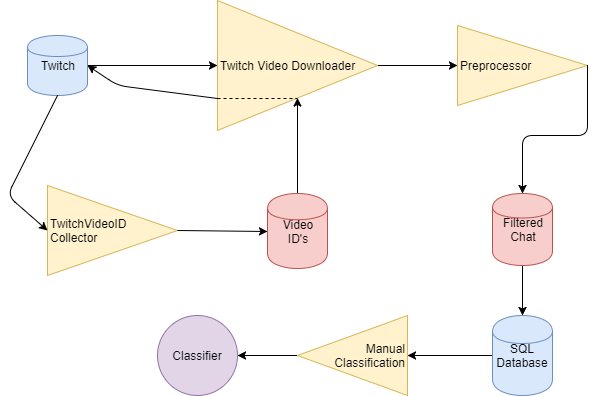
\includegraphics[width=\textwidth]{FlowChart.png}
	\caption{Flow chart}
\end{figure}

\section{Video Downloader}
First of all, all the video's that are uploaded by the 100 most popular streamers are collected. This is stored in a file which holds the streamer, together with the id's of each video.
This is done using the TwitchVideoIDCollector script. The most popular streamers are hardcoded, but can be extended easily in case the current dataset is not large enough for our goals.

After all the video id's are collected, the script TwitchVideoDownloader uses this list to fetch all the video's.
Some filtering is already at place here. The rechat functionality was implemented by Twitch at 2016-02-23, so all that are published before this date is useless since we are mainly interested in the chat.
The downloader also downloaded the video which only contains audio. Later we decided to leave the video/audio, since speech recognition is still too hard.

The TwitchVideoDownloader return the following files:
\begin{itemize}
\item A thumbnail
\item A json file with metadata of the video, which contains info like audio codec, frame rate and upload date.
\item A json file with apiinfo
\item A json file with the chat
\item A mp4 with the video, which only contains audio.
\end{itemize}

A small script is used to convert all the json data to pickle format to use with python in the preprocessor script as pickle files are processed faster in python. Later it would become clear this would be obsolete as python is too slow to pre process all the data. This is described in the next section.

\section{Preprocessor}
Before we could train our classifier we must filter the chat.
The chat is filled with emotes and ascii art which is not supported by our trainer/classifier.
At first we started off with a python script which removed each word in TwitchEmotes.txt.
All detected unicode characters are removed in the same way.
The TwitchEmotes.txt file was relatively small in the beginning, so the python script could handle all the chat files fast enough.
However, later we detected there are a lot more emotes, but also custom subscriber emotes by the streamers.
This expanded our text file massively to around 104k words. 
At this point, the python script needed way to much time to filter all chat files with the new emotes list.

So we switched to $C\#$ to implement our preprocessor as this language is significantly more efficient compared to python for loops and string replacement.
This script was able to filter the chat data within 10 minutes, a major improved compared to the python script.
It was further optimized by tokenizing the string and using a key lookup in a hashset of the words to be filtered.
This processes about 200 thousand to 600 thousand messages per second on one core.
This in comparison to about 1500 to 6000 messages per second on 16 cores by using the python implementation.
Now the filtered data is ready to be used to train the classifier in detecting toxicity.

\section{SpeechRecognition}
Originally we wanted to analyse the interaction between the streamer and the users, so we needed data from the streamer.
The audio downloaded was used with the python library SpeechRecognition. %https://pypi.python.org/pypi/SpeechRecognition/%.
But the time needed to analyse an audio file was around 1:1, so 1 minute of audio took 1 minute to parse. The result of the speech recognition was far from usable, returning mostly nonsense.

Different speech recognition toolkits were looked into:
\begin{enumerate}
\item Python speech recognition 3.7.1 which includes CMU Sphinx as speech recognition software. It is very slow as the processing must happen in real-time.
\item Dragon Speech Recognition Software, which is a professional software package. However it has high price which makes it not viable for our project.
\item Google Cloud Speech API, google has a free tool that can be used for speech recognition. It is however very slow like all other tools and does not return usable text.
\end{enumerate}

All the tools used work in real-time, so this means they are all very slow, likewise none of them returned usable data that doesn't contain errors.
This is expected as speech recognition is still not at the required level to properly gather reliable data, moreover music is usually played on stream and together with game sounds this interferes significantly with the speech recognition.
We conclude that speech recognition on a massive dataset is still not a viable option.
In the near future when services are cheaper and the recognition technology is more advanced it could become interesting to look into this.

\section{Training}
To analyse the chat data, we had to gather a training set in which the chat is rated based on their toxicity.
We converted the compressed pickle file to a chat log from the MLG channel to an SQL insert statement to store the chat into a MySQL database.
A website implemented in JavaScript and PHP showed this chat and we manually rated each chat message with a 1 to 5 (1 being non-toxic, 5 being very toxic).

The final training set is also filtered on words that are shorter than 3 letters to remove even more noise.

\section{Classifier}
%NLTK
The classifier downloads a sub set of the manually classified data.
Extracts word based features and trains a Naive Bayes or MaxEnt classifier.
The problem was in the initial distribution of all the classes for the classifier.
There are way too many messages rated 1 (non-toxic).
Thus the output of the classified was mostly 1.000 (float).

\end{document}